\documentclass[12pt]{article}
\usepackage{graphicx} % Required for inserting images
\usepackage{ragged2e}  % Enables justification
\usepackage{geometry}
\usepackage{caption}
\usepackage{subcaption}
\usepackage[x11names]{xcolor}
\usepackage{minted}
\usepackage{xparse}
\usepackage{wrapfig}
\usepackage{amsmath}
\usepackage{float}
\usepackage[
    backend=biber,
    style=numeric-comp,
    sorting=none
]{biblatex}
\usepackage{hyperref}
\usepackage{soul}
\usepackage{mathtools}
\usepackage{amssymb}
\usepackage{cancel}
\usepackage{dirtytalk}
\usepackage{scrextend}
\usepackage{multicol}
\usepackage{booktabs}

\addbibresource{references.bib}

\hypersetup{
    colorlinks=true,
    linkcolor=blue,
    citecolor=SpringGreen4,
    filecolor=magenta,      
    urlcolor=cyan,
    pdftitle={An Exploration of Statistical Methods in Determining the Gaussianity of LIGO Detector Data},
    pdfpagemode=FullScreen,
    }

\definecolor{shellbackground}{rgb}{0.95,0.95,0.92}

\geometry{
letterpaper,
% left=0.75in,
% right=0.75in,
left=0.8in,
right=0.8in,
top=0.8in,
bottom=0.8in
}

\begin{document}

\begin{titlepage}
  % \vspace*{1cm}
  \centering
  {\LARGE \textbf{University of Massachusetts Dartmouth}}\\[0.5cm]
  {\Large \textbf{Department of Mathematics}}\\[2cm]
  {\huge \textbf{An Exploration of Statistical Methods in Determining the Gaussianity of LIGO Detector Data}}\\[2cm]
  {\Large A Data Science project}\\[0.2cm]
  {\Large by}\\[0.2cm]
  {\Large \textbf{Ashish Thomas Mathew}}\\[0.2cm]
  {\Large (02101455)}\\[1.5cm]
  {\Large Project Advisors:}\\[0.75cm]
  {\Large \textbf{Dr. Sarah Caudill}}\\[0.2cm]
  {\Large University of Massachusetts Dartmouth}\\[0.75cm]{\Large \textbf{Dr. Melissa Lopez}}\\[0.2cm]
  {\Large National Institute for Subatomic Physics (Nikhef)}\\[1.5cm]
  {\Large Submitted in Partial Fulfillment of the}\\[0.2cm]
  {\Large Requirements for the Degree of}\\[0.2cm]
  {\Large Master of Science}\\[1.5cm]
  {\large \textbf{May, 2025}}
  \vfill
\end{titlepage}

\clearpage  % Ensure it starts on a new page
\normalfont % Reset to normal font (removes centering effects)
\raggedright % Ensure left alignment (prevents centering issues)

\begin{center}
    \Large \textbf{Abstract}  % Title formatting
\end{center}

\justifying

\noindent The Advanced Laser Interferometer Gravitational-wave Observatory (LIGO) is one of the most sophisticated instruments ever built, capable of measuring motion 10,000 times smaller than a proton. It was the first device to detect a gravitational wave (GW) event. While analyzing the GW data from LIGO, the detector noise is approximated to be stationary and Gaussian. However, due to its high sensitivity, a common issue it faces is its susceptibility to glitches: transient, non-Gaussian noise bursts that contaminate the time series data obtained from the detector. This project aims to develop a tool to test if the distribution of the amplitudes of the detector noise is Gaussian or not as a way to assess whether it is clean up to a defined threshold, hence improving the quality of the analysis performed. Taking the null hypothesis that the distribution is Gaussian, we study statistical approaches of normality testing, namely the Shapiro-Wilk test, the Kolmogorov-Smirnov test, and the Anderson-Darling test, to test this null hypothesis against the alternative of the distribution being non-Gaussian. We found that of the three tests, the Shapiro-Wilk test performed the best in detecting non-Gaussian samples with an accuracy of 73.86\% and a precision of 91.67\%. In comparison, the Kolmogorov-Smirnov test had an accuracy of 64.43\% and a precision of 100\%, while the Anderson-Darling test had an accuracy of 63.9\% and a precision of 100\% when detecting non-Gaussianity. 

% (The results of this project show that statistical hypothesis testing can be an effective tool for detecting glitches in LIGO detector data, and can be used as a fast alternative to the current methods used in the field. The results also show that the Shapiro-Wilk test is the most effective of the three tests studied, and can be used as a reliable tool for detecting non-Gaussian samples in LIGO detector data.)

\section{Introduction}\label{Introduction}

\noindent Nearly a century after Einstein's prediction of the existence of gravitational waves (GWs) in 1916, the first direct gravitational wave detection was achieved by the Advanced Laser Interferometer Gravitational-Wave Observatory (aLIGO) \cite{Abbott_LIGO_2016} and Virgo \cite{Accadia_virgo_2012} interferometers during the binary black hole merger event GW150914 on September 14, 2015. The LIGO Livingston (L1) interferometer underwent several upgrades following this run - effectively a massive redesign - enhancing its sensitivity by 15\% to 25\% \cite{grant_advanced_2016}. This improvement was evident during the O2 observing run during which L1, in conjunction with its Hanford (H1) counterpart and Virgo (V1), detected eleven new gravitational wave signals \cite{collaboration_gwtc-1_2019}. Subsequently, during the O3 run, all three detectors operated at their best possible sensitivity, leading to the first single-detector GW detection, GW190425, achieved by LIGO Livingston \cite{abbott_gwtc-2_2021}. There have been over 90 GW events recorded at a high level of confidence since the LIGO-Virgo collaboration's inception to date \cite{collaboration_gwtc-3_2023}.

\medskip
\noindent A consequence of these detectors' sensitivities is their susceptibility to noise. During observation runs, various noise sources, such as seismic noise, suspension thermal noise, and sensing noise, affect the data collected by the interferometers. Among these, the most problematic are \textbf{glitches}: transient events caused by non-astrophysical phenomena such as anthropogenic noise, weather conditions, or instrument malfunctions \cite{collaboration_guide_2020, collaboration_characterization_2016}. Glitches manifest as localized bursts of excess power in interferometer time series data and often do not have well-defined sources. They can occur at energy levels and frequencies that overlap with GW signals, thereby mimicking them and increasing the number of false positive detections. During the first half of the third observing run (O3a) H1 and L1 recorded glitches rates of $0.29\text{ min}^{-1}$ and $1.10\text{ min}^{-1}$ respectively, which rose to $0.32\text{ min}^{-1}$ and $1.17\text{ min}^{-1}$ during the second half (O3b) \cite{collaboration_gwtc-3_2023}. A notable example of glitches posing such an issue was during the binary neutron star merger event GW170817 \cite{collaboration_gw170817_2017}, during which instrumental noise transients were detected before the event's coalescence time, complicating its detection and subsequent analysis.

\medskip
\noindent This project aims to develop a tool to test if the amplitudes of detector noise in a sample of data from the detector contains a glitch through tests of \textbf{Gaussianity}. Gaussianity is the property of a sample distribution of data being normally distributed, also known as a Gaussian distribution. A normal/Gaussian distribution is a continuous probability distribution for a random variable where most of the data points are located around the mean, with lesser amounts of data further away. The Gaussian distribution is symmetric about the mean $\mu$, which is equal to zero, with the standard deviation $\sigma$ being equal to 1. This distribution is important as it can approximate many real world phenomena, such as the distribution of heights and weights of a country's population. It is also the basis for many statistical tests and methods. Any variation from this distribution is considered non-Gaussian. Figure \ref{fig:gaussian_distribution} shows an example of a Gaussian distribution.

\begin{figure}[H]
    \centering
    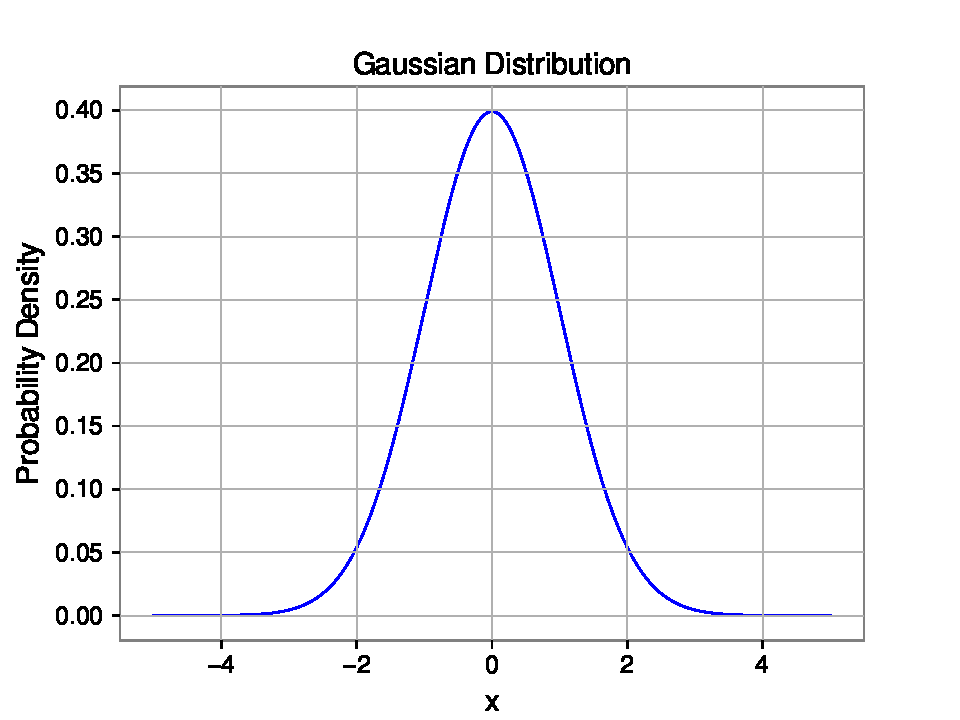
\includegraphics[width=0.55\textwidth]{images/gaussian_distribution.pdf}
    \caption{Example of a Gaussian distribution}
    \label{fig:gaussian_distribution}
\end{figure}

% The probability density function (PDF) of this distribution is given by

% \begin{equation}
%   f(x) = \frac{1}{\sqrt{2 \pi \sigma^2}} e^{-\frac{(x - \mu)^2}{2 \sigma^2}}
%   \label{eq:normal_distribution}
% \end{equation}

% \medskip
% \noindent  To study this, the Fourier transformed samples of the data are taken into account. In the case of Gaussian noise, the real and imaginary parts of the Fourier transformed parts of the noise are independent and identically distributed (i.i.d.) random variables, with a mean of 0 and a variance of $\sigma^2$. The Fourier transformed data can be modeled as a complex Gaussian distribution, which is a generalization of the normal distribution to complex numbers. The real and imaginary parts of the Fourier transformed data are normally distributed, and their joint distribution is given by

% \medskip
% \noindent The number of clean samples obtained from this process is significantly lower than the number of glitch samples. This is because the LIGO detectors are highly sensitive and are often affected by noise events, leading to fewer segments of clean data to work.

\medskip
\noindent All the noise sources in a detector collectively produce time series signals which can be treated as stochastic processes with their corresponding joint probability distributions and statistical properties \cite{collaboration_guide_2020}. In gravitational wave data analysis the noise floor of the detectors is approximated to be stationary and Gaussian. In the event of a glitch, the noise has some structure with a high signal-to-noise ratio (SNR), making it \textit{non-Gaussian}. 

\medskip
\noindent This study uses three tests of Gaussianity, namely, (1) the Shapiro-Wilk test, (2) the Kolmogorov-Smirnov test, and (3) the Anderson-Darling test on preprocessed samples of the L1 interferometer data to determine their normality and assess how well these tests differentiate between Gaussian and non-Gaussian samples. This experiment also includes studying the distributions, durations, and frequency ranges, with particular emphasis on failure points for each statistical test across various glitch types. Furthermore, considering the frequency bands at which each glitch type occurs, this study also examines how each statistical test performs under band-pass filtering at various frequency ranges.

\medskip
\noindent Another aspect of this project is the exploration of statistical hypothesis testing on time-amplitude domain data as a faster alternative to the current glitch detection methods working in the time-frequency domain. Detecting and mitigating the effects of glitches in interferometric strain data remains an active area of research within astrophysical data analysis, with several techniques proposed and implemented for the same \cite{robinet_omicron_2020, MACLEOD2021100657, davis_subtracting_2022}. However, many of these are computationally expensive, slowing down the process of assessing of the signals for glitch activity. The more popular solutions incorporate the \textit{Q-transform} \cite{chatterji_multiresolution_2004, vazsonyi_identifying_2023}, a modification of the standard Fourier transform where the analysis window scales inversely with frequency. The Q-transform is used as inputs to statistical tests to obtain a p-value depicting the statistical significance of excess power in the data. Assuming the background data to be Gaussian, the excess power that does not follow a Gaussian distribution suggests the presence of a glitch. While this method is effective for post-detection run analysis, it is much slower when scaled up to work on multiple samples. Figures \ref{fig:qtransform_vs_windowsize} and \ref{fig:qtransform_vs_samplecount} illustrate the time taken to compute the Q-transform while varying the sample window size and the number of samples respectively. 

\begin{figure}[H]
  \centering
  \begin{subfigure}[t]{0.65\textwidth}
    \centering
    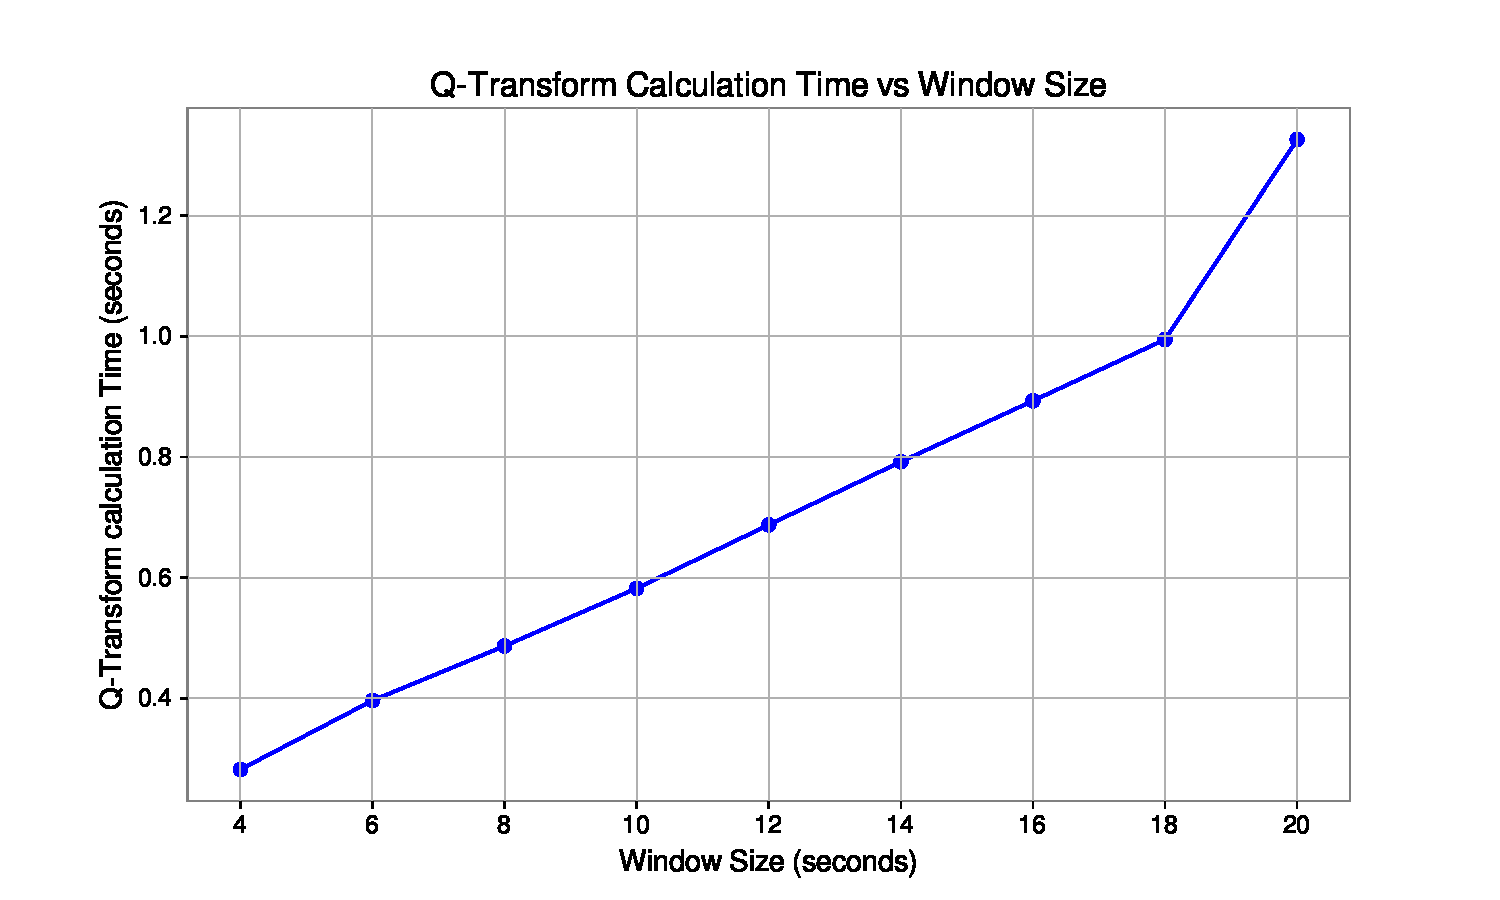
\includegraphics[width=\textwidth]{images/q_transform_time_vs_window_size.pdf}
    \caption{A plot of the Q-transform calculation time against the sample window for a single  }
    \label{fig:qtransform_vs_windowsize}
  \end{subfigure}
  \hspace{25px}
  \begin{subfigure}[t]{0.65\textwidth}
    \centering
    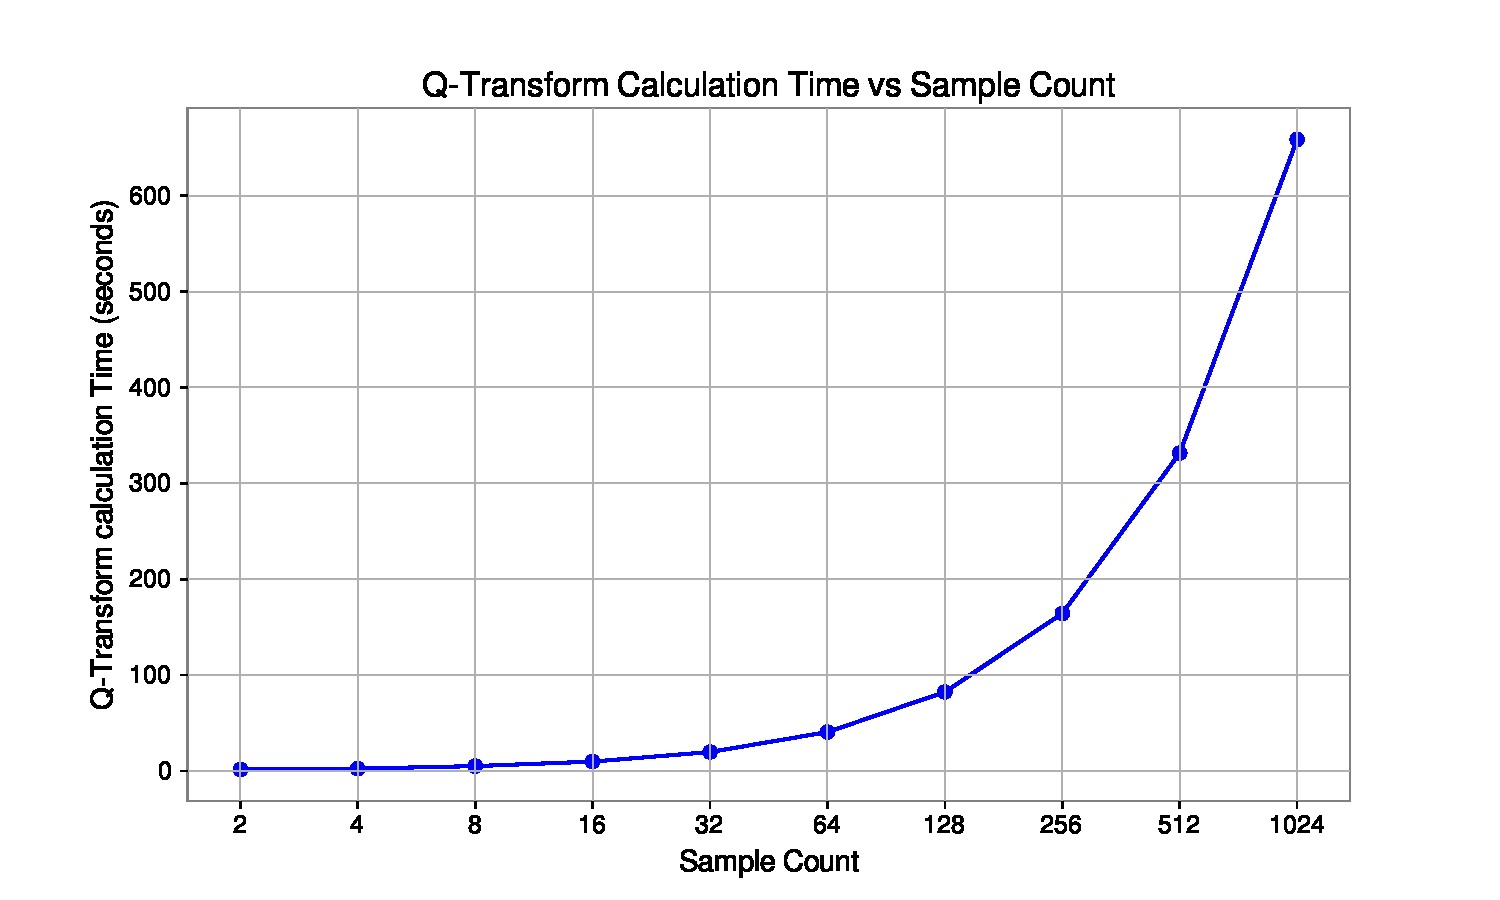
\includegraphics[width=\textwidth]{images/q_transform_time_vs_sample_count.pdf}
    \caption{Interference pattern}
    \label{fig:qtransform_vs_samplecount}
  \end{subfigure}
  \caption{Illustrations of a basic Michelson interferometer \cite{Stannered_Interferometer_2007,wiredsense_michelson_guide} and what an interference pattern would look like.}
\end{figure}

\noindent This report is organized as follows: Section \ref{Data} discusses how interferometer data is obtained and describes the properties of the time series data used in this study. It also outlines the process of acquiring clean and glitched samples and the preprocessing applied. Section \ref{Methods} describes in detail the statistical tests of Gaussianity used to assess the sample data. The experimental procedures and results are presented in Sections \ref{Experiment_1} and \ref{Experiment_2}. Finally, Section \ref{Conclusions} summarizes the findings of our experiments, discussing the strengths and limitations of the methods.

\pagebreak

\section{Data Acquisition and Conditioning}\label{Data}

\medskip
\noindent The Advanced LIGO and Virgo interferometers are large-scale, heavily modified versions of the Michelson interferometer (Figure \ref{fig:interferometer}), originally invented by American physicist Albert A. Michelson in 1887 \cite{weiss_report_1972,collaboration_gwtc-3_2023}. LIGO operates in a vacuum, using a laser beam of light split into two orthogonal parts with the help of a half-silvered mirror mounted on horizontal seismometer suspensions. The orthogonally split beams are then sent through two arms of the interferometer, known as Fabry-Pérot cavities. Each of these arms is 4 kilometers long, consisting of mirrors at each end. The first of the mirrors is fixed in place, while the second one is movable with the help of precise micrometer drives. The laser beams, when reflected by the mirrors on either end of the arms, are combined again at the beam splitter and sent to photoelectric detectors.

\medskip
\noindent The advanced LIGO interferometer is designed such that if the beams travel equal distances, the recombination would lead to a destructive interference pattern, resulting in no light coming out of the instrument \cite{ligo_what_interferometer}. When a disturbance of either astrophysical or terrestrial origin is detected, an infinitesimally small change occurs in lengths of the detector arms, in the order of $10^{-8}m$ \cite{ghonge_assessing_2024}. One of the arms is stretched, and the other arm is compressed in the perpendicular direction, altering the lengths of the reflected and combined beams, misaligning them and resulting in an interference pattern (Figure \ref{fig:sinusoidal_fringes}). This interference pattern, coupled with results from several other sensors, provides detailed information on the \textit{strain} of the GW or glitch event being observed.

\begin{figure}[H]
  \centering
  \begin{subfigure}[t]{0.4\textwidth}
    \centering
    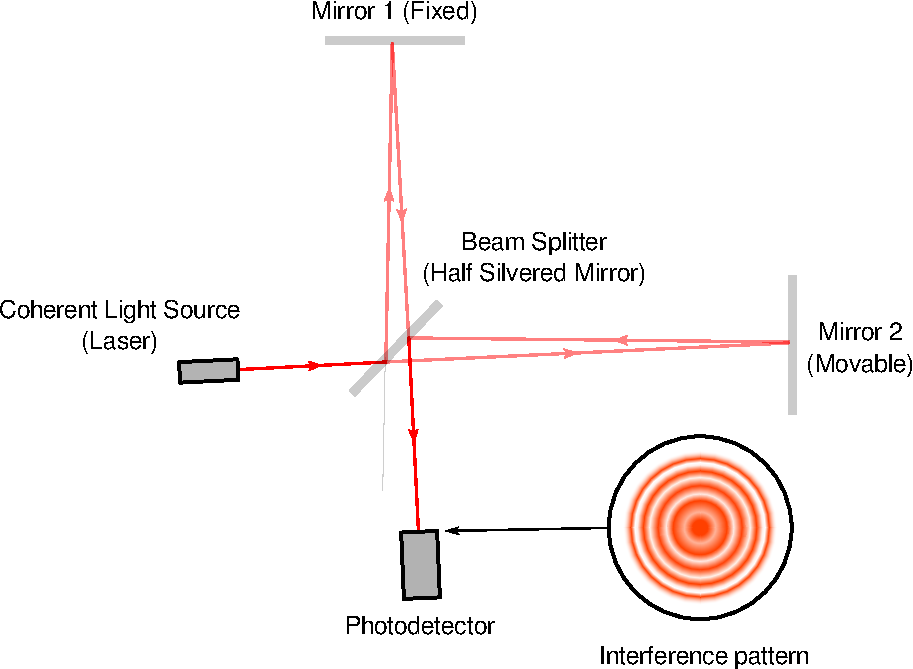
\includegraphics[width=\textwidth]{images/interferometer.pdf}
    \caption{Construction of an Interferometer}
    \label{fig:interferometer}
  \end{subfigure}
  \hspace{25px}
  \begin{subfigure}[t]{0.25\textwidth}
    \centering
    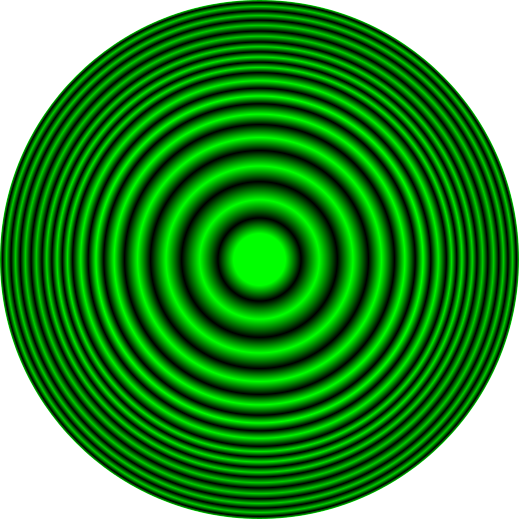
\includegraphics[width=\textwidth]{images/interference_pattern.png}
    \caption{Interference pattern}
    \label{fig:sinusoidal_fringes}
  \end{subfigure}
  \caption{Illustrations of a basic Michelson interferometer \cite{Stannered_Interferometer_2007,wiredsense_michelson_guide} and what an interference pattern would look like.}
\end{figure}

\noindent The \texttt{GWpy} Python package is widely used in this project. It provides a suite of tools to access and condition detector strain data from the Gravitational-Wave Open Science Centre (GWOSC) database \cite{gwpy}. This data is in the time domain, as timestamps in the GPS time system at nanosecond precision, and records the amplitude of the calibrated noise event as a differential change in lengths of the interferometer arms. GWpy handles detector data using the \texttt{TimeSeries} object, which is built upon \texttt{numpy} arrays. This allows compatibility with most of the core numpy utilities along with custom functions for signal processing, tabular data filtering, and visualization.

\medskip
\noindent We use the strain data from L1 during O3a for this project due to the high rate of occurrence of glitches. Figure \ref{fig:data_acq_cond} shows the steps taken to acquire signal data from the detector and condition it for statistical testing.

\begin{figure}[H]
    \centering
    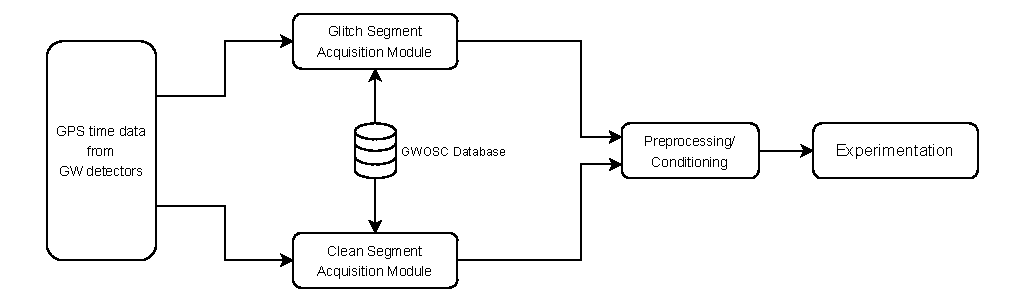
\includegraphics[width=\textwidth]{images/data_acquisition_preparation.pdf}
    \caption{The Data Acquisition and Conditioning Pipeline}
    \label{fig:data_acq_cond}
\end{figure}

\medskip
\noindent There are two main types of detector samples that we receive from the detectors: \textbf{Glitched detector data} and \textbf{Clean detector data} with separate modules used to obtain them.

\subsection{The Glitch Segment Acquisition Module}\label{Glitchdata}

\medskip
\noindent The \textbf{Glitch Segment Acquisition Module} uses GPS times of glitch occurrences obtained from \textit{Gravity Spy} \cite{Zevin_2017} to fetch our glitch samples from the GWOSC database. GravitySpy is a large-scale citizen-science project that combines astrophysics, machine learning, and human efforts to classify glitches in GW interferometer data. The \textit{Omicron} transient search algorithm is used by Gravity Spy to generate q-transform spectrograms and calculate the SNR of the time series samples \cite{robinet_omicron_2020}. This algorithm is crucial in identifying the most useful samples for data classification and analysis. Based on the morphological characteristics from the spectrograms, a total of 22 glitch classes were identified with an SNR above 7.5 and peak frequencies between 10 Hz and 2048 Hz.

\medskip
\noindent In the O3a data for L1, Fast\_Scattering and Tomte glitches are the most prevalent, while Chirp, 1080Lines and Wandering\_line glitches have fewer samples, as shown in Table \ref{tab:glitch_classes}. The No\_Glitch class represents glitch samples that lack significant traits or energy levels and do not fit in with the other classes morphologically. Hence, for our study, we do not consider this glitch class.

% \noindent\makebox[\textwidth]{%
\begin{table}[H]
    \centering
    \begin{tabular}{lr|lr}
    \toprule
    Glitch Class & Count & Glitch Class & Count \\
    \midrule
    Fast\_Scattering & 21749 & Whistle & 896 \\
    Tomte & 18708 & Low\_Frequency\_Lines & 788\\
    Blip\_Low\_Frequency & 7549 & Scratchy & 207 \\
    Scattered\_Light & 5398 & Repeating\_Blips & 164 \\
    No\_Glitch & 5358 & Violin\_Mode & 164 \\
    Extremely\_Loud & 4319 & Paired\_Doves & 155 \\
    Koi\_Fish & 4268 & Light\_Modulation & 72 \\
    1400Ripples & 2363 & Helix & 21 \\
    Blip & 1947 & Wandering\_Line & 20 \\
    Power\_Line & 1189 & 1080Lines & 9 \\
    Low\_Frequency\_Burst & 1187 & Chirp & 6 \\
    \bottomrule
    \end{tabular}
    \caption{Glitch counts per class for LIGO Livingston (L1) during the O3a run.}
    \label{tab:glitch_classes}
\end{table}

\medskip
\noindent The time series samples of the glitches are obtained using the \texttt{TimeSeries.fetch\_open\_data()} API provided by GWpy. When querying the API, a sample rate of 4096 Hz is used and a padding of 10 seconds is taken on either side of each of the glitch GPS time to obtain the beginning and end times of the window for preprocessing the glitch. This is done to ensure that the sample being used is large enough for data conditioning.

\subsection{The Clean Segment Acquisition Module}\label{Cleandata}

\noindent The \textbf{Clean Segment Acquisition Module} is used to both, find the start and end times of the gaps of clean detector noise as well as obtain the corresponding time series data. This is done using \texttt{gwtrigfind}, a package developed to search for event triggers files from GW detectors, in conjunction with \texttt{EventTable} and \texttt{TimeSeries.fetch\_open\_data()}, provided by GWpy.

\medskip
\noindent Taking the start and end GPS times of the O3a run, gwtrigfind is used to find the file path containing Omicron triggers from the \textit{L1:GDS-CALIB\_STRAIN} channel of the L1 detector. EventTable is then used to load all the trigger data, containing information on the start and end GPS times of the events. Taking the time frames between the end and start times of successive events, we obtain the start and end times of the gaps between glitches/GW triggers, which do not have a significant amount of noise activity. The sizes of the gaps are clamped between 7 and 30 seconds because too short of a gap could lead to the inclusion of glitches in the sample, as the time series data may not have enough time to stabilize after a glitch. Additionally, a short time segment would affect the PSD calculation and subsequent preprocessing. Too long of a time gap could be indicative of detector malfunction or a period of time when it is not operational.

\medskip
\noindent The start and end GPS times of the clean segments are then used to calculate their Q-transform and corresponding p-values. The GPS time intervals with a p-value greater than 0.05 are considered to be clean segments of data.

\medskip
\noindent To obtain the time series samples, similar to the glitch data, the GWOSC database is queried by taking the beginning and ending GPS times as the limits and a sample rate of 4096 Hz.

\medskip
\noindent The clean and glitched GPS times from the glitch and clean segment acquisition modules are saved as CSV files. This allows them to be used for procuring the time series samples from GWOSC without having to go through the acquisition of the segments again.

\subsection{Data Preprocessing/Conditioning}\label{DataConditioning}

\noindent The strain readings obtained from a GW detector are usually a combination of the GW signal and detector noise \cite{cutler_gravitational_1994, moore_gravitational-wave_2015, Li:2013lza}. Given our focus on the noise, it is important to bring out its characteristics such that it can be visually observed and studied. Considering the strain output to be $s(t)$ with $n(t)$ as the noise and $h(t)$ being the possible signal received, the GW detector output is given by:

\begin{equation}
    s(t) = n(t) + h(t)
    \label{eq:strain_output}
\end{equation}

\medskip
\noindent The preprocessing in this project, which was mentioned in previous section and will be discussed in sections \ref{PSD_ASD} and \ref{Whitening}, involves the use of Fourier transforms. Given the signal $x(t)$ in the time domain we get its corresponding Fourier transform in the frequency domain $\tilde{x}(f)$ as

\begin{equation}
    \tilde{x}(f) = \mathcal{F}\{ x(t) \} (f) = \int_{-\infty}^{\infty} x(t) e^{-2 \pi i f t} dt
    \label{eq:fourier_transform}
\end{equation}

\medskip
\noindent and the inverse Fourier Transform given by

\begin{equation}
  x(t) = \mathcal{F}^{-1} \{ \tilde{x}(f) \} (t) = \int_{-\infty}^{\infty} \tilde{x}(f) e^{2 \pi i f t} df
  \label{eq:inverse_fourier_transform}
\end{equation}

\subsubsection{Power Spectral Density and Amplitude Spectral Density}\label{PSD_ASD}

% \noindent The noise in the GW detectors is approximated to be stationary \cite{collaboration_characterization_2016}, i.e. the characteristics of the noise do not change over time, and the components are, for the most part, uncorrelated, hence keeping it Gaussian. As a result, the statistical properties of the noise can be described by an auto-correlation matrix described by

% $C_n(\tau)$
% \begin{equation}
%     C_n(\tau) = \langle n_a(t+\tau) n_b(t) \rangle - \langle n_a(t+\tau) \rangle \langle n_b(t) \rangle,
%     \label{eq:autocorrelation}
% \end{equation}

% \medskip
% \noindent Where $\langle \cdot \rangle$ represents the ensemble average The Wiener-Khinchin theorem \cite{chatfield1989analysis} states that the Fourier transform of the correlation matrix of a signal gives us the \textbf{power spectral density} (PSD) $S_n(f)$. This would give us the following equation:

% \begin{equation}
%   S_n(f) = 2 \int_{-\infty}^{\infty} C_n(\tau) e^{-2 \pi i f \tau} d\tau \\
%   S_n(f) = 2 \tilde{C_n}(\tau) \\
%   \label{eq:psd_autocorrelation}
% \end{equation}

\noindent One of the  methods to study the glitch signal is the \textbf{Power Spectral Density (PSD)}. The PSD, provides a representation of how power is distributed across different frequency bands in a noise signal\cite{Oppenheim_2009}, allowing for the identification of dominant frequency components and their corresponding amplitudes. Assuming the noise sources to be non-stationary and taking the frequency domain representation of the noise signal $n(f)$, the ensemble average of the Fourier components is given by \cite{Li:2013lza}

\begin{equation}
  \langle \tilde{n}(f) \tilde{n}^*(f') \rangle = \frac{1}{2} \delta(f - f') S_n(f).
  \label{eq:psd_relation}
\end{equation}

\medskip
\noindent Where, $\langle \cdot \rangle$ represents the ensemble average, $\tilde{\cdot}$ represents the Fourier transform from \ref{eq:fourier_transform}, $\cdot^\ast$ represents the complex conjugate, and $S_n(f)$ is the PSD. Aside from PSD, another way to characterize the noise of a detector is with the \textbf{Amplitude Spectral Density (ASD)} values, given by

\begin{equation}
  ASD(f) = \sqrt{S_n(f)}
\end{equation}

\noindent The ASD measures the amplitude of the signal at each frequency, and it is often used to compare the noise levels of different detectors or to assess a detector's sensitivity to specific frequencies. The ASD is normally plotted on a logarithmic scale, with frequency on the x-axis and the ASD on the y-axis, allowing for easy identification of noise peaks and their corresponding frequencies.

\begin{figure}[H]
  \centering
  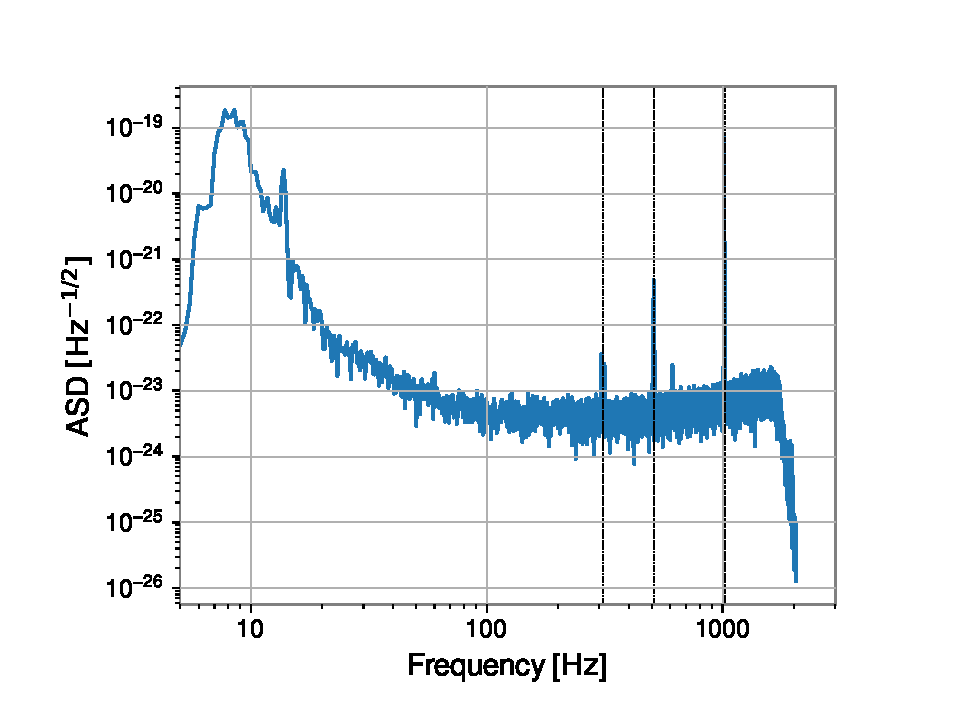
\includegraphics[width=0.6\textwidth]{images/unwhitened_asd.pdf}
  \caption{ASD plot for a Tomte Glitch. The gray dotted lines coincide with strong spectral lines at around the 300, 512, and 1024 Hz ranges, marked by dotted lines. There is a big chance that these are of instrumental origin.}
  \label{fig:asdtomte}
\end{figure}

\medskip
\noindent From figure \ref{fig:asdtomte}, which shows an example Tomte glitch ASD plot, to obtain the root-mean-square strain noise at a given frequency band, we integrate over the squares of the ASD readings over the frequency band of interest and take its square root. The problem with ASD plots, however, is that it does not visually capture the glitch signal well enough because they are relatively weak, highly transient and easily overpowered by the instrument noise. To better visualize the glitch, we would instead choose to \textbf{whiten} the time series data and experiment with it in the time-amplitude domain.

% Todo: Add plots comparing glitch and clean ASD

\subsubsection{Whitening}\label{Whitening}

\textbf{Whitening} is the process of suppressing low-frequency and spectral line noise from the data to allow for a clearer view of the underlying signals at sensitive frequency ranges. Whitening is one of the first steps in GW data analysis. By whitening the data, we effectively reduce the impact of noise on our analysis, improving the sensitivity of our detection methods.

\medskip
\noindent Whitening is done by taking the inverse of the estimated ASD and multiplying it with the Fourier coefficients of the original time series data \cite{collaboration_guide_2020}.

\begin{align}
    \tilde{n}_\text{whitened}(f) = \frac{\tilde{n}(f)}{ASD} = \frac{\tilde{n}(f)}{\sqrt{S_n(f)}} \\
    n_\text{whitened}(t) = \mathcal{F}^{-1} \left\{ \tilde{n}_\text{whitened}(f) \right\}
    \label{eq:whitening}
\end{align}

\medskip
\noindent This effectively flattens the power across all frequencies, allowing for a clearer view of the glitch signal. The resulting whitened data can then be used for further analysis, such as statistical testing or machine learning classification.

\medskip
\noindent In figure \ref{fig:sampletomte} we see a Tomte glitch signal before and after whitening. In the first plot we do not clearly see the effects of the glitch on the time series data. However, after whitening the data, we can clearly see the glitch signal in the time-amplitude plot. The Q-transform allows a view of the non-stationary portion of the glitch signal, which shows a clear peak in the normalized energy coinciding with the glitch event. For a clean signal we would not see any significant peaks in the whitened time series or non-stationary parts in the Q-transform.

\medskip
\noindent In this project, the data from the clean and glitch segment acquisition modules are whitened using the method. After whitening, the glitch samples are cropped to a 0.5 second time window around the GPS time of the glitch event, effectively giving us a 1 second glitch sample to work with. The clean data, in turn, is divided into 1 second segments, each being treated as a separate clean sample for statistical testing.

\begin{figure}[H]
  \centering
  
\includegraphics[width=0.6\textwidth]{images/sample_plot.pdf}
  \caption{Example of a Tomte glitch signal before and after whitening.}
  \label{fig:sampletomte}
\end{figure}

\section{Methods}\label{Methods}

% We propose a  The null hypothesis ($h_0$) in this project is that the sample distributions being studied are Gaussian, indicating that the signal is clean. The alternative hypothesis ($h_1$) is that the distribution is non-Gaussian.

Our main objective is to determine the Gaussianity of time series data obtained from L1 and use this as a criterion to determine the presence of a glitch in it. 

\medskip
\noindent If a sample is found to be non-Gaussian, this indicates an excess of power at certain frequencies due to which there is a high chance of a glitch being present. In the previous section, we have seen how whitening the time series data brings out the glitch characteristics. Taking the same example as before, if we were to treat this whitened data as a population of points and plot the distribution, we notice that it contains heavier tails, hence making it non-Gaussian. Similarly, when observing a sample of clean data, the signal is closer to that of a Gaussian distribution. Hence, we propose a pair of hypotheses to determine the presence of a glitch in a sample of data from the detector.

% TODO: Add images for clean and glitched signal distributions. Also compare with normal distribution.

\medskip
\noindent\fbox{
  \begin{minipage}{0.97\textwidth}
    \textbf{Null Hypothesis ($H_0$):}

    Considering a sample of whitened time series detector data, if the distribution of the amplitudes is Gaussian, then the sample does not contain a glitch, i.e. the sample is clean.
  \end{minipage}
}
\\
\noindent\fbox{
  \begin{minipage}{0.97\textwidth}
    \textbf{Alternative Hypothesis ($H_1$):}

    Considering a sample of whitened time series detector data, if the distribution of the amplitudes is non-Gaussian, then the sample contains a glitch.
  \end{minipage}
}

\medskip
\noindent We employ three statistical tests of normality to test these hypotheses: the Shapiro-Wilk test, the Kolmogorov-Smirnov test, and the Anderson-Darling test. Each of these have their own strengths and weaknesses, and are used to assess the normality of the data in different ways. These tests give us a statistic along with a p-value, the latter of which will be used to determine the significance of the result. The p-value tells us how strongly the statistic rejects the null hypothesis. For our tests, a low p-value indicates that the sample data is unlikely to be Gaussian, hence indicating the presence of a glitch. The significance level for our tests, $\alpha$, is set to 0.05, which tells us that if the p-value is less than it, we reject the null hypothesis and accept the alternative hypothesis.

% \noindent This allows us to better understand the results, as they provide a direct measure of their significance. For example, if we took the Kolmogorov-Smirnov test, the calculated statistic is a distance measure, which can be difficult to interpret in terms of the distribution being Gaussian or not. The p-value, on the other hand, gives us a direct measure of the probability of the test statistic being as extreme as calculated hence, eliminating the need to determine a critical value for each statistic. Additionally, setting different critical values for each test would lead to vastly different results, making it difficult to compare the results. The p-values standardize the results hence allowing for like-to-like comparison of the result.

\medskip
% \noindent If the p-value is less than a predetermined significance level, 0.05 in this case, we reject the null hypothesis and conclude that the sample data is not normally distributed, hence containing a glitch. Appendix \ref{pvalues} discusses p-values and the discourse and reasoning behind the selection of the 0.05 threshold.

% \medskip
% \noindent For our use case, the null hypothesis $H_0$ is that the sample data contains a glitch non-Gaussian/ not normally distributed, while the alternative hypothesis $H_1$ is that the sample data is Gaussian. As we will see in the following sections, this is the inverse of the null hypothesis for the statistical tests being used This is so that we can determine the effectiveness of these tests as glitch detection tools.

\subsection{The Shapiro-Wilk Test}\label{ShapiroWilk}

The Shapiro-Wilk test \cite{Shapiro1965} is a parametric test, meaning that it assumes the data follows a specific distribution. This parametric test follows the idea of calculating a test statistic $W$ based on the ratio of the best estimate of the sample data's variance to its actual variance. This was the first test that could detect departures from normality due to either the skewness or the kurtosis of the data.

\medskip
\noindent\textbf{Skewness} is a measure of asymmetry of a distribution. It indicates how much the data deviates either to the left or right from a symmetric distribution. A skewness of 0 indicates a perfectly symmetric distribution, while positive and negative values indicate a right and left skew respectively. \textbf{Kurtosis}, on the other hand, measures the tails of the distribution, indicating how much of the data is contained in the tails compared to a normal distribution. A kurtosis of 3 indicates a normal distribution, while values greater than 3 indicate heavier tails and values less than 3 indicate lighter tails.

\medskip
\noindent If we were to consider $x_1, x_2, \ldots, x_n$, to be a collection of ordered sample points from a population, ranked smallest to largest, with the sample mean $\bar{x}$ and $a_1, a_2, \ldots, a_n$ being constants computed from the expected values of the order statistics of a normal distribution, then the test statistic $W$ is given by:

\begin{equation}
    W = \frac{(\sum\limits_{i=1}^{n} a_i x_{(i)})^2}{\sum\limits_{i=1}^{n} (x_i - \bar{x})^2}
    \label{eq:shapiro_wilk_statistic}
\end{equation}

\medskip
\noindent Taking $m = (m_1, m_2, \ldots, m_n)$ to be the expected values of the order statistics of a normal distribution such that $m_i = \mathbb{E}[z_i]$ where $z_i$ is the $i$-th order statistic of the normal distribution, and $V$ the covariance matrix of the ordered statistics, the constants $a_i$, which make up the \textbf{optimal weight vector} $a \in \mathbb{R}^n$, can be computed as

\begin{align}
    a_i &= \frac{m^T V^{-1}}{||V^{-1} m||} \\
        &= \frac{m^T V^{-1}}{(m^T V^{-1}V^{-1}m)^{1/2}}
    \label{eq:shapiro_wilk_constants}
\end{align}

\medskip
\noindent The test statistic $W$ lies in the range $[0, 1]$, with values closer to 1 indicating that the sample data is more likely to be Gaussian. The null hypothesis $H_0$ is rejected if $W$ is significantly less than 1, indicating that the sample data is non-Gaussian.

\medskip
\noindent The p-value of the statistic is usually used to determine the significance of the result. If the p-value is less than the significance level defined, the null hypothesis is rejected, indicating that the sample data is non-Gaussian and likely contains a glitch.

\medskip
\noindent The Shapiro-Wilk test, though powerful, has some limitations. It is sensitive to the sample size and may not perform well with small or large samples. It works ideally for sample sizes $n \leq 2000$. The \texttt{shapiro()} function from \texttt{scipy.stats} works well for $n \leq 5000$ after which the p-value calculations' accuracy drops. Additionally, for this test to work the data must be continuous and univariate.

\subsection{The Kolmogorov-Smirnov Test}\label{KolmogorovSmirnov}

The Kolmogorov-Smirnov (KS) test is a non-parametric test, originally proposed in the 1930s, used to decide whether a sample comes from a particular type of distribution \cite{Kolmogorov_1951, chakravarti1967}. The idea of this test is to check the difference in shape between the distributions being studied, which is done by measuring the maximum vertical distance between the \textbf{empirical cumulative distribution function (ECDF)} of the sample and the \textbf{cumulative distribution function (CDF)} of the reference distribution, which in this case is a Gaussian distribution. This test has two versions: the \textbf{one-sample KS test} which is used to compare an empirical sample distribution with a reference theoretical distribution, and the \textbf{two-sample KS test} which compares the empirical distributions of two samples. We use the one-sample KS test in this project.

% TODO: Add EDF and CDF comparison image
\begin{figure}[H]
    \centering
    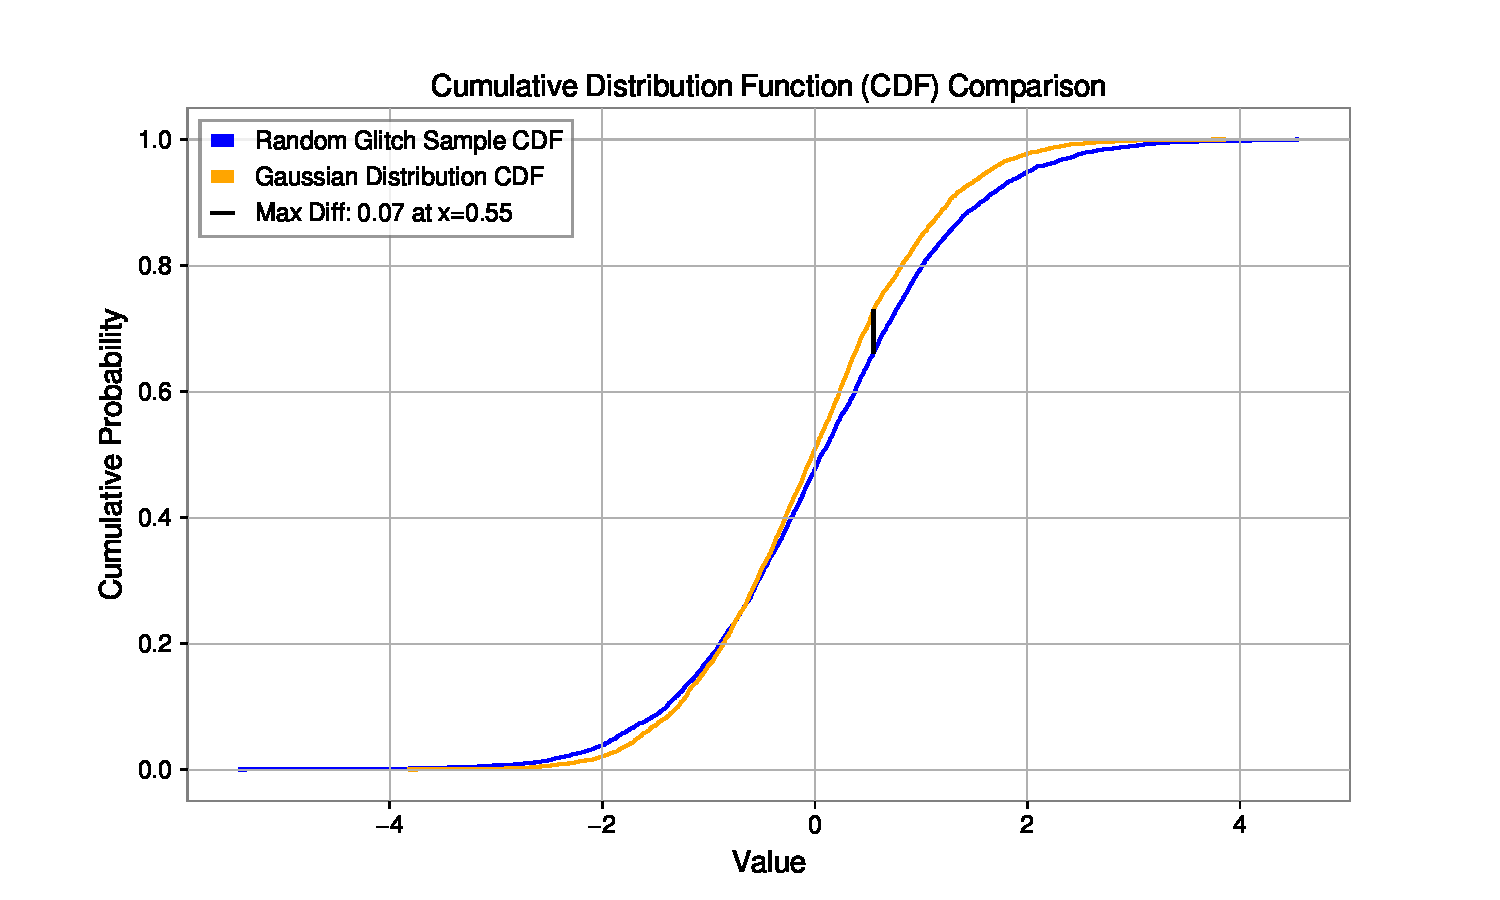
\includegraphics[width=0.8\textwidth]{images/cdf_comparison_glitch_gaussian.pdf}
    \caption{The KS statistic calculation for a sample glitch against a Gaussian distribution. The black line is the maximum absolute difference between the sample glitch CDF and the Gaussian CDF, which is the KS statistic $D_n$.}
    \label{fig:ecdf_cdf_comparison}
\end{figure}

\medskip
\noindent  Taking a sample of ordered points $X_1, X_2, \ldots, X_N$ as $N$ ordered points from a population, the Empirical CDF of the sample, is given by

\begin{equation}
    F_N = \frac{n(i)}{N}
    \label{eq:edf}
\end{equation}

\medskip
\noindent Where $n(i)$ is the number of points less than or equal to $X_i$ in the sample. This is in the form of a step function increasing at steps of $1/N$ at each ordered point \cite{guthrie_nistsematech_2020}. Taking the theoretical CDF of the distribution being tested as $F$s, a Gaussian distribution in our case, the KS test statistic $D_n$ is defined as

\begin{equation}
    D_n = \sup_{1 \leq i \leq N} \left( F(X_i) - \frac{i - 1}{N} , \frac{i}{N} - F(X_i) \right)
    \label{eq:ks_statistic}
\end{equation}

\medskip
\noindent Here,  $\text{sup}$ refers to the supremum or maximum of the differences between the theoretical CDF and the ECDF. If $D_n$ is significantly larger than the critical value, it indicates that the sample data significantly differs from a Gaussian distribution, hence rejecting the null Hypothesis.

\subsubsection{Note: Scaling the data}\label{Scaling}

\noindent The Kolmogorov-Smirnov test, is highly affected by the values of the data. We need to ensure that the comparisons being done in the test is not affected due to the absolute values of the data points. Hence, this requires for the data to be scaled down to the same range of a standard normal distribution. This is achieved by scaling the data to have a mean of 0 and a standard deviation of 1. This is also known as \textbf{standardization} or \textbf{z-score normalization}.

\medskip
\noindent To achieve this the \texttt{StandardScaler} class from the \texttt{sklearn.preprocessing} module is used. This module works by transposing the data to have a zero mean, calculates the standard deviation, and scales the data points down such that the standard deviation is 1. The \textbf{standard score} or \textbf{z-score} of a sample point, which tells us how many standard deviations it is from the mean, is given by

\begin{equation}
    z = \frac{x - \mu}{\sigma},
    \label{eq:scaling_formula}
\end{equation}

\medskip
\noindent where $x$ is the original data point, $\mu$ is the mean, and $\sigma$ is the standard deviation of the data. The $z$ value obtained can be treated as the new data point after scaling and is particularly useful in this case as it does not change the position of the data point in its calculation.

\subsection{The Anderson Darling test}\label{AndersonDarling}

The Anderson-Darling (AD) test is a goodness-of-fit test used to determine whether a sample of data is drawn from a specific distribution, most commonly a normal distribution. It is a modification of the Kolmogorov-Smirnov and Cramer-von Mises tests with more sensitivity to differences in the tails of the distribution \cite{guthrie_nistsematech_2020, Michael_2025_statsref}.

\medskip
\noindent Similar to the Kolmogorov-Smirnov test, this test compares the ECDF of the sample data with the CDF of a theoretical reference distribution by taking a distance function between them. The main difference here is that the full range of the data is used to calculate the distance function rather than just the largest distance value \cite{Michael_2025_statsref}. Here, taking $n$ to be the number of elements in the sample and $w(x)$ to be the weighting function, the Anderson-Darling statistic distance $A^2$, given by the squared area between the sample ECDF $F_n(x)$ and the theoretical reference CDF $F(x)$, is calculated as

\begin{equation}
  A^2 = n \int_{-\infty}^{\infty} \left( F_n(x) - F(x) \right)^2 w(x) dF(x)
  \label{eq:ad_distance_function}
\end{equation}

\medskip
\noindent Taking the weighting function $w(x)$ is defined as

\begin{equation}
    w(x) = \frac{1}{F(x) (1 - F(x))}
    \label{eq:ad_weighting_function}
\end{equation}

\medskip
\noindent We get $A^2$ \cite{anderson1954test} as

\begin{equation}
    A^2 = n \int_{-\infty}^{\infty} \frac{\left( F_n(x) - F(x) \right)^2}{F(x)(1 - F(x))} \; dF(x)
    \label{eq:ad_statistic_distance_updated}
\end{equation}

\medskip
\noindent To obtain random samples from a distribution function, the CDF is to be calculated and random samples $x$ are to be taken from a uniform distribution $x \in [0, 1]$. Hence, the Anderson-Darling test statistic can be rewritten as

\begin{equation}
    A^2 = -N -S
    \label{eq:ad_statistic}
\end{equation}

\medskip
\noindent where $S$ is given by

\begin{equation}
  S =  \frac{1}{N} \sum\limits_{i=1}^{N} \left( 2i - 1 \right) \left( \ln F(X_i) + \ln (1 - F(X_{N-i+1})) \right)
  \label{eq:ad_statistic_full}
\end{equation}

\medskip
\noindent hence, giving us the final form of the Anderson-Darling statistic as

\begin{equation}
  A^2 = -N - \sum\limits_{i=1}^{N} \left( \frac{2i - 1}{N} \right) \left( \ln F(X_i) + \ln (1 - F(X_{N-i+1})) \right)
  \label{eq:ad_statistic_full}
\end{equation}

\noindent This is effectively a weighted cross-product of the samples, allowing for a comparison of the sample data with the reference distribution.

\medskip
\noindent In the case of the mean and standard deviation of the sample distribution being known with the distribution size, $N$ being greater than $5$, the significance levels are $1\%$, $2.5\%$, $5\%$, $10\%$ and $15\%$, with the critical values for each significant level being pre-computed through Monte-Carlo simulations. The null hypothesis is rejected if the calculated statistic is greater than the critical value at a selected significance level, indicating that the sample data is not normally distributed.

\medskip
\noindent Along with studying how effective these tests are at determining the Gaussianity of GW detector data, we will also be validating the claim in \cite{razali2011power}, which states that the Shapiro-Wilks test is the most powerful, followed by the Anderson darling test and the Kolmogorov-Smirnov test.


% Cramer-Von Mises test (It is a part of the Anderson-Darling test so it might not be needed)
% KL- Divergence
% Jarque-Bera test
% D'agostino's K-squared test
% Bispectrum test - 3rd order cumulant
% Trispectrum test - 4th order cumulant
% Coefficient of Variation Envelope

\pagebreak
\section{Experimentation}\label{Experimentation}

The implementation of our statistical tests on the whitened time series data is fairly straightforward, with the \texttt{scipy.stats} package providing dedicated functions for each. Once the time series data for the clean and glitch samples are obtained and conditioned, their amplitude values are directly used as inputs to the following functions to obtain the relevant statistics and p-values.

\begin{itemize}
  \item \texttt{scipy.stats.shapiro()} for the Shapiro-Wilk test
  \item \texttt{scipy.stats.ks\_1samp()} for the one-sample Kolmogorov-Smirnov test
  \item \texttt{scipy.stats.anderson()} for the Anderson-Darling test
\end{itemize}

\medskip
\noindent The results of these tests are compared against the significance level of 0.05 to determine whether the null hypothesis is rejected or not.

\subsection{Using the complete frequency range}\label{Experiment_1}

\subsection{Using a band pass filter}\label{Experiment_2}
% No of samples, how to recreate the tests we did

% Jarque-Bera test

%  TODO: Discussions

\section{Conclusion}\label{Conclusions}


% The p-value is the probability of observing a test statistic as extreme as the one calculated, assuming that the null hypothesis is true. If the p-value is less than a predetermined significance level (commonly 0.05), we reject the null hypothesis and conclude that the sample data is not normally distributed.


% Bibliography
% Acknowledgements
% Appendix

% Describe whitening

% \begin{figure}[H]
%   \centering
%   \begin{subfigure}[t]{0.35\textwidth}
%     \centering
%     \includegraphics[width=\textwidth]{images/me.jpg}
%     \caption{A picture of me}
%     \label{fig:me}
%   \end{subfigure}
%   ~
%   \begin{subfigure}[t]{0.35\textwidth}
%     \centering
%     \includegraphics[width=\textwidth]{images/quantized_me.jpg}
%     \caption{Me, but quantized to a factor of 1}
%     \label{fig:me_quantized}
%   \end{subfigure}
%   \caption{An example of how quantization leads to banding in images}
% \end{figure}


% \begin{minted}[
% frame=lines,
% framesep=2mm,
% baselinestretch=1.2,
% bgcolor=Cornsilk2,
% fontsize=\footnotesize,
% linenos
% ]{Python}
% factor = # An integer factor determined by the user
% for each row from top to bottom:
%     for each column from left to right:
%         oldpixel = image[column][row]

%         # Quantizing the current pixel and calculating the error
%         newpixel = quantize(oldpixel, factor)
%         image[column][row] = newpixel
%         quantization_error = oldpixel - newpixel

%         # Spreading the quantization error to the surrounding pixels
%         image[column+1][row]   = clamp(image[column+1][row]   + (quantization_error*7/16))
%         image[column+1][row+1] = clamp(image[column+1][row+1] + (quantization_error*1/16))
%         image[column][row+1]   = clamp(image[column][row+1]   + (quantization_error*5/16))
%         image[column+1][row-1] = clamp(image[column+1][row-1] + (quantization_error*3/16))

% function quantize(pixel, factor):
%     return round(factor * pixel/255.0) * 255/factor

% # This function prevents the color values from going above 255 or below 0
% function clamp(value):
%     return max(0, min(value, 255))
% \end{minted}

% \begin{figure}[H]
%     \centering
%     \includegraphics[width=0.30\textwidth]{images/RGB_color_gradient_100x100.png}
%     \caption{The Original Image}
%     \label{fig:confirmation_image}
% \end{figure}

% \begin{figure}[h]
%   \centering
%   \begin{subfigure}[t]{0.30\textwidth}
%     \centering
%     \includegraphics[width=\textwidth]{images/dithered_RGB_color_gradient_100x100.png}
%     \caption{Serial Dithering Result}
%     \label{fig:serial_dithering_confirmation}
%   \end{subfigure}
%   ~
%   \begin{subfigure}[t]{0.30\textwidth}
%     \centering
%     \includegraphics[width=\textwidth]{images/parallel_dithered_RGB_color_gradient_100x100.png}
%     \caption{Parallel Dithering Result}
%     \label{fig:parallel_dithering_confirmation}
%   \end{subfigure}
%   \caption{A comparison of the dithering results from our serial and parallel codes.}
% \end{figure}

\printbibliography[title={References}]


\end{document}
